%! TeX program = lualatex
% Converted from book/ch8.md by book/tools/md2tex.py (initial conversion).
% This .tex file is the maintained source from now on; the converter is kept for provenance only.
% CONVERSION NOTE: graphicx's trim= option takes four space-separated lengths; the markdown had commas, which LaTeX rejects.
% CONVERSION NOTE: restored every mangled `\```{math}` back to `\\[` (a line break with vertical space)
\documentclass[../book.tex]{subfiles}
\begin{document}

\chapter{Systems of Differential Equations}\label{ch:sys}

We already know that many biological phenomena are multidimensional. In this chapter we expand our ability to create and analyse multi-dimensional models by learning to develop and solve coupled systems of differential equations. In coupled systems of differential equations, the solution to one equation depends on the solution to another and (possibly) vice versa. As you will see, we will have to draw on our previous experience with both calculus and vectors in order to untangle the recursive statements with which we are faced.

Counter-intuitively, we will begin our discussion by exploring a non-linear system of differential equations intended to model the dynamics of a predator species and its prey.  The model, itself, was originally proposed as part of an effort to understand the oscillatory ``boom and bust'' patterns seen in certain fisheries, and it highlighted how cycles seen in natural populations can be driven by endogenous factors.

\section{Predator-prey dynamics}

Consider two populations of species whose dynamics are coupled by the fact that one is preyed upon by the other. Let \(n_1(t)\) and \(n_2(t)\) denote the number of individuals in the prey and predator populations, respectively, at time \(t\). We will assume that both populations are cut off from migration, and we model the population dynamics using conservation laws that pay attention only to births and deaths.

In an effort to keep our model as simple as possible, we will assume the per-capita birth rate of the prey species is a constant, \(\alpha>0\). Thus, the total rate birth rate of the prey population is \(\alpha n_i(t)\). We will also assume that mortality among prey is primarily due to predation. To capture this, we model the per-capita death rate of the prey species as \(\beta  n_2(t)\), where \(\beta >0\) is a constant. In this case, if there are no predators, our model predicts no death among prey. It follows that the total death rate of the prey species is \(\beta n_2(t) n_1(t)\), and so
\begin{subequations} \label{eq:system}
  \begin{equation} \label{eq:prey}
    \frac{dn_1(t)}{dt} = \alpha  n_1(t) - \beta  n_1(t) n_2(t)
  \end{equation}
  is the net rate of production in the prey population.

  Our model for the dynamics of the predator population will also be simple. We assume that the prey species is the main food source for the predator, and use \(\gamma n_1(t)\), with \(\gamma >0\) constant, to describe the per-capita birth rate of the predator. Here, if there are no prey species present, then the birth rate of the predator is zero. We model the per-capita death rate of the predator as a constant, \(\delta >0\). It follows that
  \begin{equation} \label{eq:predator}
    \frac{dn_2(t)}{dt} = \gamma  n_1(t) n_2(t) - \delta  n_2(t)
  \end{equation}
\end{subequations}
is the net rate of production in the predator population.

The equations \eqref{eq:prey} and \eqref{eq:predator} form a coupled system because the solution to one depends on the solution to the other. We can express this coupled system simply as \(\vec{n}^{ \prime}(t) = \vec{F}(\vec{n}(t))\), where
\begin{equation}\label{eq:sys-1}
\vec{F}(\vec{n}(t))
=
\begin{bmatrix}
  \left( \alpha  - \beta  n_2(t)\right) n_1(t) \\
  \left( \gamma  n_1(t) - \delta\right) n_2(t)
\end{bmatrix}
\end{equation}
is a non-linear vector field. Recognizing that we can think of the system of differential equations as a vector field is helpful because it can give us hints about the solutions.

Let's think about sketching the vector field to get a better sense of what solutions to the system \eqref{eq:system} might look like. We will sketch the vector field by applying \(\vec{F}(\vec{n})\) to the point corresponding to \(\vec{n}\) in the positive quadrant of \(n_1,n_2\)-space. To help us out, we will make reference to two lines: the horizontal line \(n_2 = \frac{\alpha}{\beta}\), the vertical line \(n_1 = \frac{\delta}{\gamma}\).

When \(\vec{F}\) is applied to points above the aforementioned horizontal line, its first element, namely \(\frac{dn_1}{dt}\), is negative. This is due to the fact that \(n_2 > \frac{\beta}{\alpha}\). On the other hand, when \(\vec{F}\) is applied to points below the aforementioned horizontal line, its first element is positive owing to the fact that \(n_2 < \frac{\beta}{\alpha}\). Of course, if \(\vec{F}\) is applied to a point directly on the horizontal line, \(n_2 = \frac{\beta}{\alpha}\) and so its first element is zero.

Let's now turn our attention to the aforementioned vertical line. When \(\vec{F}\) is applied to the right (respectively, the left) of said line, its second element, namely \(\frac{dn_2}{dt}\), is positive (respectively, negative) because \(n_1 > \frac{\delta}{\gamma}\) (respectively, \(n_1 < \frac{\delta}{\gamma}\)). If \(\vec{F}\) is applied a point directly on the vertical line, the fact that \(n_1 = \frac{\delta}{\gamma}\) means that its second component is zero.

We can put all the information presented above together to get a composite sketch of \(\vec{F}\) in \(n_1,n_2\)-space. As we see in Figure \ref{fig:predprey1} the vector field suggests anticlockwise rotation in this two-dimensional space. Because \(\vec{n}^{ \prime}(t) = \vec{F}(\vec{n}(t))\), the vector field is tangent to the solutions to \eqref{eq:system}, at least when those solutions are projected into \(n_1,n_2\)-space. Therefore, we expect the solutions to rotate in \(n_1,n_2\)-space as well. This rotation means that, when expressed as functions of time, solutions will oscillate with numbers rising and falling repeatedly as time goes on.

\begin{figure}[htbp]
  \centering
  \missingfigure{../standalones/build/plot-predprey1.pdf}
  \caption{A very rough sketch of the vector field \(\vec{F}(\vec{n})\). Direction of arrows suggests anticlockwise rotation, but further analysis is required. The arrows lead us to predict that the solution to \eqref{eq:system}, projected into \(n_1,n_2\)-space, will also rotate in an anticlockwise manner, possibly as shown by the purple curve.}
  \label{fig:predprey1}
\end{figure}

As Figure \ref{fig:predprey1} shows, when we project the solutions to system \eqref{eq:system} into \(n_1\) and \(n_2\) it is tempting to view one variable as a function of the other. If we take that perspective, then we might conjecture that curves, like the purple one in Figure \ref{fig:predprey1}, satisfy
\begin{equation}\label{eq:sys-2}
\frac{dn_2}{dn_1}
=
\frac{(\gamma n_1(t) - \delta )n_2(t)}{(\alpha - \beta n_2(t) ) n_1(t)}.
\end{equation}
Note that this new differential equation has been constructed by dividing the predator equation in \eqref{eq:predator} by prey equation in \eqref{eq:prey}.

With a little algebra, the preceding equation becomes
\begin{equation}\label{eq:sys-3}
\frac{\alpha - \beta n_2(t) }{n_2(t)}  \frac{dn_2}{dn_1}
=
\frac{\gamma n_1(t) - \delta }{n_1(t)}.
\end{equation}
Next, integrating with respect to \(n_1\) gives us
\begin{equation}\label{eq:sys-4}
\int
\frac{\alpha - \beta n_2}{n_2}  \frac{dn_2}{dn_1} dn_1
=
\int
\frac{\gamma n_1 - \delta }{n_1} dn_1
\end{equation}
which, after an elementary change of variable on the left, becomes
\begin{equation}\label{eq:sys-5}
\int
\frac{\alpha - \beta n_2}{n_2} dn_2
=
\int
\frac{\gamma n_1 - \delta }{n_1} dn_1.
\end{equation}
Completing the integration shown, and keeping in mind that \(n_1\) and \(n_2\) are both strictly postive, we arrive at
\begin{equation}\label{eq:relation}
  \alpha \ln n_2 - \beta n_2 = \gamma  n_1 - \delta  \ln n_1 +C
\end{equation}
where \(C\) is a constant. We cannot solve this equation to express one variable as a function of the other. However, we can look at the equation as a relation between \(n_1\) and \(n_2\). Moreover, we can represent that relation as a curve, with different values of \(C\) defining different curves.\footnote{Like the way in which we represent \(x^2 + y^2 = C\), for positive \(C\), as a circle of radius \(\sqrt{C}\).} When we plot our relation between \(n_1\) and \(n_2\), we see that it takes a rather odd shape, but does yield a closed curve in the plane (Figure \ref{eq:fieldplot}).

\begin{figure}
  \begin{center}
    \includegraphics[scale=0.5,trim={1in 4.5in 2in 0.75in}, clip]{standalones/plot-predPrey.pdf}
    \parbox{4.5in}{
      \caption{The dynamics of the prey population (\(n_1\)) and the predator population (\(n_2\)) are revealed when we plot the relation in equation \eqref{eq:relation}. Curves  were constructed assuming \(\alpha = 3\), \(\beta = \gamma = \frac{3}{2}\), and \(\delta = 1\). Curves correspond to different values of the constant \(C\), and are overlaid on the vector field associated with the system of differential equations in \eqref{eq:system}. If we think of the current state of the populations as a particle (``\(\bullet\)''), then that particle will travel along the curve, periodically returning to its original position. The significance of points A-D is made clear in the text.  \label{eq:fieldplot} }
    }
  \end{center}
\end{figure}

Using Figure \ref{eq:fieldplot} we can deduce key qualitative predictions of our predator-prey model. First, the fact that curves are closed means that the dynamics are predicted to be periodic. This means that at some time in the future the populations will simultaneously return to their current state.

Second, the shape of each closed curve means that the oscillations we expect to see in species' population sizes will be out of phase. As an example of this, suppose the population began with a relatively moderate number of prey and a relatively small number of predators (at point A in Figure \ref{eq:fieldplot}). From there, numbers of prey and predator will increase until the system reaches point B in Figure \ref{eq:fieldplot}. Beyond point B, numbers of prey will begin to fall, but numbers of predators will continue to increase. The size of the predator population would be greatest as the system passes through point C in Figure \ref{eq:fieldplot}. Between points C and D in Figure \ref{eq:fieldplot} both populations decline in size, then prey begin to recover as the system passes through point D.

\begin{figure}
  \begin{center}
    \includegraphics[scale=0.55]{standalones/plot-time_series.pdf}
    \parbox{4.5in}
    {
      \caption{ Solution to system \eqref{eq:system} presented as functions of time. Predator and prey numbers oscillated, in agreement with Figure \ref{eq:fieldplot}. \label{fig:time_series}}
    }
  \end{center}
\end{figure}

If we modify numerical methods we encountered in an earlier chapter, we can generate a solution to \eqref{eq:system}, as shown in Figure \ref{fig:time_series}. That solution confirms the oscillatory behaviour we have just described. The solution also raises two concerns. One is that the predator population is often larger than the prey population, which runs counter to what we see in many ecosystems. Admittedly, this prediction is likely the result of poor choices for parameters \(\alpha\), \(\beta\), \(\gamma\) and \(\delta\) and not a limitation of the model itself. The second concern, however, is a bit more substantive and relates to the fact that, given certain initial conditions, the model predicts that population sizes drop well below \(1\) for a reasonable period of time. This concern has been dubbed the \emph{attofox problem}, since the model will predict that even populations with \(10^{-18}\) individuals eventually recover. The attofox problem suggests that the predictions of our deterministic model break down and should be replaced by ones generated by model that incorporates uncertainty.

\section{Linear Systems of Differential Equations}
Before one can analyse models of biological phenomena based around non-linear systems of differential equations, one must first come to terms with linear ones. In this chapter, we will define a \emph{linear system of differential equations} as a collection of equations of the form
\begin{equation}\label{eq:sys-6}
\begin{array}{ccc}
  \dfrac{du_1}{dt} 
              &=&
              a_{11} u_1(t) + \cdots + a_{1n} u_n(t) 
              + 
              b_1(t) 
              \\
              &\vdots & 
              \\
              \dfrac{du_n}{dt}
              &=&
              a_{n1} u_1(t) + \cdots + a_{nn} u_n(t) 
              + b_n(t) 	
\end{array}
\end{equation}
where \(a_{11}, \ldots, a_{1n}, \ldots, a_{n1}, \ldots a_{nn}\) are real constants, and \(b_1(t), \ldots, b_n(t)\) are given functions of the variable \(t\). In matrix-vector notation, we can re-write the previous system as
\begin{equation}\label{eq:sys-7}
\frac{d\vec{u}}{dt} = A \vec{x} + \vec{b}(t)
\end{equation}
where \(A\) is the matrix whose \(ij\)th entry is the constant \(a_{ij}\) and \(\vec{b}(t)\) is the vector whose \(i\)th entry is \(b_i(t)\).

In this chapter, we will restrict our discussion to systems of two equations with \(\vec{b}(t)\) independent of \(t\). Consequently, \(A\) will be a \(2\times 2\) matrix and \(\vec{b}\) will be a vector containing two constants. Though the Exercises provided below do present you with the occasional three-dimensional system, sensible modifications of the presentation surrounding two-dimensional problems can be applied to find solutions.

Our discussion will begin by focusing on systems for which \(\vec{b} = \vec{0}\). In keeping with terminology introduced in Chapter 2, such systems are called \emph{homogeneous} and stand apart from \emph{inhomogeneous} systems where \(\vec{b}\neq \vec{0}\).

Consider the following homogeneous equation
\begin{equation}\label{eq:sys-8}
\frac{d}{dt}
\begin{bmatrix}
  x_1(t) \\ \vdots \\ x_n(t)
\end{bmatrix}	 
= 
\begin{bmatrix}
  \lambda_1 &\cdots& 0 \\
  \vdots & \ddots & \vdots \\
  0&\cdots& \lambda_n
\end{bmatrix}
\begin{bmatrix}
  x_1(t) \\ \vdots \\ x_n(t)
\end{bmatrix}	 
\end{equation}
where the only non-zero entries of the matrix are found on the diagonal. This system is easy to solve because the equations are not coupled

\subsection{Homogeneous systems: distinct real eigenvalues}

Consider the initial-value problem suggested by
\begin{equation}\label{eq:sys-9}
\frac{d\vec{u}(t)}{dt} = A \vec{u}(t), \quad 
\text{with}\quad \vec{u}(0) = \vec{u}_0 
\end{equation}
where \(A\) is a \(2\times 2\) matrix of constants. For the moment, we assume that \(A\) has two distinct real eigenvectors, \(\lambda_1\) and \(\lambda_2\), associated with eigenvectors \(\vec{v}_1\) and \(\vec{v}_n\), respectively. Because \(\lambda_1 \neq \lambda_2\), we can express the solution we are looking for as a linear combination of their eigenvectors as follows:
\begin{equation}\label{eq:lc1}
  \vec{u}(t)
  =
  c_1(t) \vec{v}_1 
  +
  c_2(t) \vec{v}_2.
\end{equation}
Substituting this linear combination into the differential equation gives us
\begin{equation}\label{eq:sys-10}
\begin{array}{lcl}
  \dfrac{d c_1(t)}{dt}  \vec{v}_1
  +
  \dfrac{d c_2(t)}{dt}  \vec{v}_2
      &=& 
      c_1(t) A \vec{v}_1 
      +
      c_2(t) A \vec{v}_2
      \\[1ex]
      &=&
      c_1(t) \lambda_1 \vec{v}_1 
      +
      c_2(t) \lambda_2 \vec{v}_2
\end{array}
\end{equation}
where we have used the fact that \(A \vec{v}_i = \lambda_i  \vec{v}_i\) to simplify. If we now equate the coefficients of \(\vec{v}_i\) on either side of the equation, we obtain
\begin{equation}\label{eq:sys-11}
\frac{dc_i(t)}{dt} = c_i(t) \lambda_i  
\quad
\text{for } i = 1, 2
\end{equation}
which is easily solved to give
\begin{equation}\label{eq:sys-12}
c_i(t) = c_i(0) e^{\lambda_i  t}
\quad
\text{for } i = 1,2.
\end{equation}
After putting this expression for \(c_i(t)\) into \eqref{eq:lc1}, we arrive at a solution to the given initial-value problem:
\begin{equation} \label{eq:lc2}
  \vec{u}(t) = c_1(0) e^{\lambda_1  t}  \vec{v}_1
  +
  c_2(0) e^{\lambda_2  t} \vec{v}_2.
\end{equation}
It can be shown ours is the only solution to the initial-value problem given, in the case where \(A\) has distinct real eigenvalues. However, proving that is beyond the scope of this book.

In words, equation \eqref{eq:lc2} tells us that the solution to the initial value problem is a linear combination of the \emph{fundamental solutions}  \(e^{\lambda_i  t} \vec{v}_i\). Once we identify the fundamental solutions, the coefficients used to combine them -- namely \(c_1(0)\) and \(c_2(0)\) -- are found by using information given by the initial condition. The next example illustrates this point.

\begin{example} \label{eg:DE-linear1}
Solve the following initial-value problem:
\begin{equation}\label{eq:sys-13}
\begin{array}{lcl}
  u_1'(t) &=& u_2(t) - 2 u_1(t) \\
  u_2'(t) &=&  u_1(t) + 2 u_2(t) 
\end{array}
\quad
\text{with}
\quad
\begin{array}{lcl}
  u_1(0) &=& 2\sqrt{5}, \\
  u_2(0) &=& -2\sqrt{5}.
\end{array}
\end{equation}
\end{example}
\begin{solution}
We can re-write the given problem as \(\vec{u}^{ \prime}(t) = A \vec{u}(t)\), where
\begin{equation}\label{eq:sys-14}
A =
\begin{bmatrix}
  -2 & 1 \\ 1 & 2
\end{bmatrix}.
\end{equation}
The eigenvalues of the matrix are \(\lambda_1 = \sqrt{5}\) and \(\lambda_2=-\sqrt{5}\). These are real and distinct, and so the formula we developed can be used to solve the problem.

The eigenvector \(\vec{v}_1 = \begin{bmatrix} 1 \\ \sqrt{5}+2 \end{bmatrix}\) is a member of the family associated with \(\lambda_1=\sqrt{5}\), and the eigenvector \(\vec{v}_2 = \begin{bmatrix} 1 \\ -\sqrt{5}+2 \end{bmatrix}\) is a member of the family associated with \(\lambda_2 = -\sqrt{5}\). It follows that the fundamental solutions are
\begin{equation}\label{eq:sys-15}
e^{\lambda_1  t}  \vec{v}_1
=
e^{t\sqrt{5}} 
\begin{bmatrix}
  1 \\ \sqrt{5}+2
\end{bmatrix}
\quad \text{and} \quad
e^{\lambda_2  t}  \vec{v}_2
=
e^{-t\sqrt{5}} 
\begin{bmatrix}
  1 \\ -\sqrt{5}+2
\end{bmatrix}.
\end{equation}

We now turn our attention to the initial conditions and solve
\begin{equation}\label{eq:sys-16}
\begin{array}{rccrccr}
                          & c_1(0) & + & & c_2(0) &=& 2\sqrt{5} \\[1ex]
  (\sqrt{5}+2) &c_1(0) & + & (-\sqrt{5}+2) & c_2(0) &=&
  -2\sqrt{5}
\end{array}
\end{equation}
to find
\begin{equation}\label{eq:sys-17}
c_1(0) = \sqrt{5}-3,\quad\text{and}\quad
c_2(0) = \sqrt{5}+3.
\end{equation}
Using our formula, then, we assert that
\begin{equation}\label{eq:sys-18}
\vec{u} (t)
=
(\sqrt{5}-3) 
e^{t\sqrt{5}}  
\begin{bmatrix}
  1 \\ \sqrt{5}+2
\end{bmatrix}
+
(\sqrt{5}+3) 
e^{-t\sqrt{5}}  
\begin{bmatrix}
  1 \\ -\sqrt{5}+2
\end{bmatrix}
\end{equation}
or equivalently
\begin{equation}\label{eq:sys-19}
\begin{array}{lcl}
  u_1(t)
                          &=&
                          (\sqrt{5}-3)  e^{t\sqrt{5}} + 
                          (\sqrt{5}+3)  e^{-t\sqrt{5}}
                          \\[1ex]
                          u_2(t)
                          &=&
                          (\sqrt{5}-3)(\sqrt{5}+2)  e^{t\sqrt{5}} + 
                          (\sqrt{5}+3)(-\sqrt{5}+2)  e^{-t\sqrt{5}}
\end{array}
\end{equation}
is the solution to the problem.
\end{solution}

We can plot the solutions to the previous problem as functions of \(t\) (Figure \ref{fig:timeseries1}). We can also project the solutions into \(u_1,u_2\)-space, which better illustrates the steps we took to arrive at a solution (Figure \ref{fig:eg_illustrate}).

Recall that we began developing our answer by finding the fundamental solutions \(e^{\lambda_i  t} \vec{v}_i\). As Figure \ref{fig:eg_illustrate} shows, these fundamental solutions trace our straight lines in the plane that are collinear with the eigenvector upon which they are based. As their name suggests, fundamental solutions satisfy the given differential equation, but do not necessarily satisfy the given initial condition. When the real eigenvalue that makes up part of a  the fundamental solution is positive, the fundamental solution, itself, flows away from the origin. By contrast, the fundamental solution flows toward the origin when the corresponding real eigenvalue is negative.

\begin{figure}[htbp]
  \centering
  \missingfigure{../standalones/build/plot-timeseries1.pdf}
  \caption{The solution to the initial-value problem in Example \ref{eg:DE-linear1}, plotted as functions of \(t\).}
  \label{fig:timeseries1}
\end{figure}

Once we found the fundamental solutions, we used them in linear combination to express the solution to the initial-value problem. In a sense, the fundamental solutions act like a skeleton on which we hang the solution we are actually focused on finding (Figure \ref{fig:eg_illustrate}).

\begin{figure}
  \begin{center}
    \begin{tikzpicture}[scale=0.4]
      \draw[variable=\r,domain=0:2,blue]
      plot( {\r*cos(deg(-0.2318238040))}, {\r*sin(deg(-0.2318238040))} );
      \draw[variable=\r,domain=0:2,blue]
      plot( {\r*cos(deg(-0.2318238040)+180)}, {\r*sin(deg(-0.2318238040)+180)} );
        %
      \draw[<-,variable=\r,domain=2:4,blue]
      plot( {\r*cos(deg(-0.2318238040))}, {\r*sin(deg(-0.2318238040))} );
      \draw[<-,variable=\r,domain=2:4,blue]
      plot( {\r*cos(deg(-0.2318238040)+180)}, {\r*sin(deg(-0.2318238040)+180)} );
        %
      \draw[<-,variable=\r,domain=4:6,blue]
      plot( {\r*cos(deg(-0.2318238040))}, {\r*sin(deg(-0.2318238040))} );
      \draw[<-,variable=\r,domain=4:6,blue]
      plot( {\r*cos(deg(-0.2318238040)+180)}, {\r*sin(deg(-0.2318238040)+180)} );
        %
      \draw[<-,variable=\r,domain=6:8,blue]
      plot( {\r*cos(deg(-0.2318238040))}, {\r*sin(deg(-0.2318238040))} );
      \draw[<-,variable=\r,domain=6:8,blue]
      plot( {\r*cos(deg(-0.2318238040)+180)}, {\r*sin(deg(-0.2318238040)+180)} );
        %
      \draw[<-,variable=\r,domain=8:10,blue]
      plot( {\r*cos(deg(-0.2318238040))}, {\r*sin(deg(-0.2318238040))} );
      \draw[<-,variable=\r,domain=8:10,blue]
      plot( {\r*cos(deg(-0.2318238040)+180)}, {\r*sin(deg(-0.2318238040)+180)} ) node[above right] {\(e^{-t\sqrt{5}}\vec{v}_2\)};
        %
        %
      \draw[->,variable=\r,domain=0:2,blue]
      plot( {\r*cos(deg(1.338972522))}, {\r*sin(deg(1.338972522))} );
      \draw[->,variable=\r,domain=0:2,blue]
      plot( {\r*cos(deg(1.338972522)+180)}, {\r*sin(deg(1.338972522)+180)} );
        %
        %
      \draw[->,variable=\r,domain=2:4,blue]
      plot( {\r*cos(deg(1.338972522))}, {\r*sin(deg(1.338972522))} );
      \draw[->,variable=\r,domain=2:4,blue]
      plot( {\r*cos(deg(1.338972522)+180)}, {\r*sin(deg(1.338972522)+180)} );
        %
      \draw[->,variable=\r,domain=4:6,blue]
      plot( {\r*cos(deg(1.338972522))}, {\r*sin(deg(1.338972522))} );
      \draw[->,variable=\r,domain=4:6,blue]
      plot( {\r*cos(deg(1.338972522)+180)}, {\r*sin(deg(1.338972522)+180)} );
        %
      \draw[->,variable=\r,domain=6:8,blue]
      plot( {\r*cos(deg(1.338972522))}, {\r*sin(deg(1.338972522))} );
      \draw[->,variable=\r,domain=6:8,blue]
      plot( {\r*cos(deg(1.338972522)+180)}, {\r*sin(deg(1.338972522)+180)} );
        %
      \draw[variable=\r,domain=8:10,blue]
      plot( {\r*cos(deg(1.338972522))}, {\r*sin(deg(1.338972522))} ) node[right] {\(e^{t\sqrt{5}}\vec{v}_1\)};
      \draw[variable=\r,domain=8:10,blue]
      plot( {\r*cos(deg(1.338972522)+180)}, {\r*sin(deg(1.338972522)+180)} );
        %
        %
        %
      \draw[->,variable=\t,domain=-0.25:-0.2,samples=10]
      plot({(sqrt(5)-3)*exp(\t*sqrt(5))+(sqrt(5)+3)*exp(-\t*sqrt(5))},
      {(sqrt(5)-3)*(sqrt(5)+2)*exp(\t*sqrt(5))+(sqrt(5)+3)*(-sqrt(5)+2)*exp(-\t*sqrt(5))} );
        %
      \draw[->,variable=\t,domain=-0.2:-0.1,samples=50]
      plot({(sqrt(5)-3)*exp(\t*sqrt(5))+(sqrt(5)+3)*exp(-\t*sqrt(5))},
      {(sqrt(5)-3)*(sqrt(5)+2)*exp(\t*sqrt(5))+(sqrt(5)+3)*(-sqrt(5)+2)*exp(-\t*sqrt(5))} );
        %
      \draw[->,variable=\t,domain=-0.15:0.1,samples=50]
      plot({(sqrt(5)-3)*exp(\t*sqrt(5))+(sqrt(5)+3)*exp(-\t*sqrt(5))},
      {(sqrt(5)-3)*(sqrt(5)+2)*exp(\t*sqrt(5))+(sqrt(5)+3)*(-sqrt(5)+2)*exp(-\t*sqrt(5))} );
        %
      \draw[->,variable=\t,domain=0.1:0.2,samples=50]
      plot({(sqrt(5)-3)*exp(\t*sqrt(5))+(sqrt(5)+3)*exp(-\t*sqrt(5))},
      {(sqrt(5)-3)*(sqrt(5)+2)*exp(\t*sqrt(5))+(sqrt(5)+3)*(-sqrt(5)+2)*exp(-\t*sqrt(5))} );
        %
      \draw[->,variable=\t,domain=0.2:0.3,samples=50]
      plot({(sqrt(5)-3)*exp(\t*sqrt(5))+(sqrt(5)+3)*exp(-\t*sqrt(5))},
      {(sqrt(5)-3)*(sqrt(5)+2)*exp(\t*sqrt(5))+(sqrt(5)+3)*(-sqrt(5)+2)*exp(-\t*sqrt(5))} );
        %
      \draw[->,variable=\t,domain=0.3:0.4,samples=50]
      plot({(sqrt(5)-3)*exp(\t*sqrt(5))+(sqrt(5)+3)*exp(-\t*sqrt(5))},
      {(sqrt(5)-3)*(sqrt(5)+2)*exp(\t*sqrt(5))+(sqrt(5)+3)*(-sqrt(5)+2)*exp(-\t*sqrt(5))} );
        %
      \draw[variable=\t,domain=0.4:0.475,samples=50]
      plot({(sqrt(5)-3)*exp(\t*sqrt(5))+(sqrt(5)+3)*exp(-\t*sqrt(5))},
      {(sqrt(5)-3)*(sqrt(5)+2)*exp(\t*sqrt(5))+(sqrt(5)+3)*(-sqrt(5)+2)*exp(-\t*sqrt(5))} ) node[below] {\(\vec{u}(t)\)};
        %
      \filldraw (4.472135954,-4.472135954) circle (0.175cm);
      \node[below right] at (4.472135954,-4.472135954) 
      {\(\begin{bmatrix} 2\sqrt{5} \\ -2\sqrt{5} \end{bmatrix}\)};
        %
      \draw[-latex, gray] (-10,0)--(10,0);
      \draw[-latex, gray] (0,-10)--(0,10);
        %\draw[gray] (-12,-12)--(12,-12)--(12,12)--(-12,12)--(-12,-12);
      \draw[dotted] (-1,-4.472135954)--(4.472135954,-4.472135954)
      --(4.472135954,-1);
    \end{tikzpicture}
    \parbox{3.75in}{
      \caption{The solution to Example \ref{eg:linear1} projected into the \(u_1,u_2\)-plane. The solution \(\vec{u}(t)\) is a linear combination of the fundamental solutions\label{fig:eg_illustrate} }
    }
  \end{center}
\end{figure}

\subsection{Homogeneous linear systems: complex eigenvalues}

The eigenvalues of a matrix are not always real, and so it is not obvious that the formula derived in the previous section can also always be used to solve problems like \(\vec{u}^{ \prime}(t) = A \vec{u}(t)\) with \(\vec{u}(0) = \vec{u}_0\) when \(A\) has complex eigenvalues. It turns out that equation \eqref{eq:lc2} still applies in this case, but some modifications are required before you might be able to use it effectively.

When \(A\) has only real entries, any complex eigenvalues it has occur as conjugate pairs \(\lambda = a+i b\) and \(\bar \lambda = a-i b\). In this case, we can simplify equation \eqref{eq:lc2}  by applying \emph{Euler's formula}. This formula says that
\begin{equation}\label{eq:sys-20}
e^{i \theta} = \cos \theta + i  \sin \theta.
\end{equation}
Euler's formula is crucial to understanding the steps that are described below.

Let \(\lambda = a+i b\) be a complex eigenvalue of \(A\), associated with the eigenvector \(\vec{v} = \vec{x} + i \vec{y}\). Then, the corresponding fundamental solution is
\begin{multline}\label{eq:sys-21}
  e^{\lambda t}
   \vec{v}
  =
  e^{(a+i b)t}  (\vec{x}+i \vec{y})
  =
  e^{a t} (\cos (bt) + i \sin (bt) )(\vec{x}+i \vec{y})
  \\[1ex]
  =
  \underbrace{
    e^{a t} ( \cos (bt) \vec{x} - \sin (bt) \vec{y} )
  }_{\text{real part}}
  +
  i 
  \underbrace{
    e^{a t} ( \sin (bt) \vec{x} + \cos (bt) \vec{y} ).
  }_{\text{imaginary part}}
\end{multline}
As we might expect, the other fundamental solution would involve \(\bar \lambda = a - i b\) and its eigenvector \(\vec{w} = \vec{x} - i \vec{y}\). With that in mind, the second fundamental solution could be expressed as
\begin{multline}\label{eq:sys-22}
  e^{\bar \lambda t}
   \vec{w}
  =
  e^{(a-i b)t}  (\vec{x}-i \vec{y})
  =
  e^{a t} (\cos (-bt) + i \sin (-bt) )(\vec{x}-i \vec{y})
  \\[1ex]
  =
  e^{a t} (\cos (bt) - i \sin (bt) )(\vec{x}-i \vec{y})
  \\[1ex]
  =
  \underbrace{
    e^{a t} ( \cos (bt) \vec{x} - \sin (bt) \vec{y} )
  }_{\text{real part}}
  -
  i 
  \underbrace{
    e^{a t} ( \sin (bt) \vec{x} + \cos (bt) \vec{y} ).
  }_{\text{imaginary part}}
\end{multline}
where we have used the fact that cosine is an even function and sine is an odd function to simplify. Following equation \eqref{eq:lc2}, we then express the solution to the initial-value problem as
\begin{multline} \label{eq:final_eq}
  \vec{u}(t)
  =
  e^{a t}
  (c_1(0) + c_2(0))
  \left(
    \cos(bt) \vec{x} - \sin(bt) \vec{y}
  \right)
  \\+
  i e^{at} (c_1(0) - c_2(0)) 
  \left(
    \sin(bt) \vec{x} + \cos(bt) \vec{y}
  \right).
\end{multline}
In this case, we allow \(c_1(0)\) and \(c_2(0)\) to be complex numbers. Given that \(\vec{u}(t)\) is a vector of real numbers, it must be the case that \(c_1(0)\) and \(c_2(0)\) in equation \eqref{eq:final_eq} are complex conjugates. With this in mind \(c_1(0) + c_2(0) = k_1(0)\) and \(i ( c_1(0) - c_2(0)) = k_2(0)\) where \(k_1(0)\) and \(k_2(0)\) are real numbers. It follows that the solution to the initial-value problem can be expressed as
\begin{equation}\label{eq:sys-23}
\vec{u}(t)
=
e^{a t} 
k_1(0)
\left(
  \cos(bt) \vec{x} - \sin(bt) \vec{y}
\right)
+
e^{at} k_2(0) 
\left(
  \sin(bt) \vec{x} + \cos(bt) \vec{y}
\right).
\end{equation}
where \(k_1(0)\) and \(k_2(0)\) are found using information provided by the initial condition \(\vec{u}(0) = \vec{u}_0\). The next example shows our modified version of \eqref{eq:lc2} at work.

\begin{example} \label{eg:complex1}
Solve the following initial-value problem:
\begin{equation}\label{eq:sys-24}
\begin{bmatrix}
  u_1'(t) \\ u_2'(t)
\end{bmatrix}
=
\begin{bmatrix}
  1 & -3 \\
  2 & 3
\end{bmatrix}
\begin{bmatrix}
  u_1(t) \\ u_2(t)
\end{bmatrix}
\quad \text{with}\quad
\begin{bmatrix}
  u_1(0) \\ u_2(0)
\end{bmatrix}
=
\begin{bmatrix}
  3 \\ 0
\end{bmatrix}.
\end{equation}
\end{example}
\begin{solution}
The eigenvalue-eigenvectors pairs for the matrix include
\begin{equation}\label{eq:sys-25}
\lambda = 2 + i \sqrt{5}, \quad
\vec{v} 
=
\begin{bmatrix}
  3 \\ -1
\end{bmatrix}
+
i 
\begin{bmatrix}
  0\\
  -\sqrt{5}
\end{bmatrix}
\end{equation}
and
\begin{equation}\label{eq:sys-26}
\bar
\lambda = 2 - i \sqrt{5}, \quad
\vec{w}
=
\begin{bmatrix}
  3 \\ -1
\end{bmatrix}
- i
\begin{bmatrix}
  0 \\ -\sqrt{5}
\end{bmatrix}
\end{equation}
Applying the formula we derived, we obtain
\begin{multline}\label{eq:sys-27}
  \begin{bmatrix}
    u_1(t) 
    \\
    u_2(t)
  \end{bmatrix}		=
  e^{2 t} 
  k_1(0)
  \left( 
    \cos (\sqrt{5} t) 
    \begin{bmatrix}
      3 \\ -1
    \end{bmatrix}
    -
    \sin (\sqrt{5} t) 
    \begin{bmatrix}
      0 \\ -\sqrt{5}
    \end{bmatrix}
  \right)
  \\[1ex]
  +
  e^{2 t} 
  k_2(0)
  \left( 
    \sin (\sqrt{5} t) 
    \begin{bmatrix}
      3 \\ -1
    \end{bmatrix}
    +
    \cos (\sqrt{5} t) 
    \begin{bmatrix}
      0 \\ -\sqrt{5}
    \end{bmatrix}
  \right)
\end{multline}
which simplifies to
\begin{multline}\label{eq:sys-28}
  \begin{bmatrix}
    u_1(t) \\ u_2(t)
  \end{bmatrix}
  =
  k_1(0) 
  e^{2t}  
  \begin{bmatrix}
    3  \cos (\sqrt{5}t)
    \\
    - \cos(\sqrt{5}t) + \sqrt{5}\sin(\sqrt{5}t)
  \end{bmatrix}
  \\[1ex]+
  k_2(0) 
  e^{2t} 
  \begin{bmatrix}
    3  \sin(\sqrt{5}t) \\
    -\sin(\sqrt{5}t) - \sqrt{5}  \cos(\sqrt{5}t)
  \end{bmatrix}.
\end{multline}
Using the given initial condition, we see that the constants \(k_1(0)\) and \(k_2(0)\) must satisfy
\begin{equation}\label{eq:sys-29}
\begin{array}{rcl}
  3  k_1(0) &=& 3 \\
  -k_1(0) - \sqrt{5} k_2(0) &=& 0
\end{array}
\end{equation}
and so \(k_1(0) = 1\) and \(k_2(0) = -\frac{1}{\sqrt{5}}\). The solution to the given problem, therefore, is
\begin{equation}\label{eq:sys-30}
\begin{array}{lcl}
  u_1(t)
                          &=&
                          e^{2 t} \left(3 \cos(\sqrt{5} t) - \frac{3}{\sqrt{5}} \sin (\sqrt{5} t)\right) \\
  u_2(t) &=&
  e^{2 t} 
  \frac{6}{\sqrt{5}}\sin(\sqrt{5}t)
\end{array}
\end{equation}
after some simplification.
\end{solution}

The solution to the previous example, plotted as a curve in the \(u_1,u_2\)-plane, shows the rotation we have come to associate with complex eigenvalues (Figure \ref{fig:complex1}). Because the real part of the eigenvalues in the example is positive, the rotational movement carries us away from the origin. Movement carries us toward the origin in those cases where the real part of the eigenvalues is negative.

\begin{figure}
  \begin{center}
    \begin{tikzpicture}[scale=0.35]
      \draw[-latex, gray] (-15,0)--(15,0);
      \draw[-latex, gray] (0,-2.5)--(0,15);
      \node[below] at (-13,13) {\(\vec{u}(t)\)};
      \filldraw (3,0) circle (0.2cm);
      \node[below right] at (3,0) {\(\begin{bmatrix} 3 \\ 0 \end{bmatrix}\)};
      \draw[variable=\t,domain=-1.5:0.2,samples=100,->]
      plot( {exp(2*\t)*( 3*cos(deg(sqrt(5)*\t)) - 3*sin(deg(sqrt(5)*\t))/sqrt(5) )},
      {exp(2*\t)*6*sin(deg(sqrt(5)*\t))/sqrt(5)} );
      \draw[variable=\t,domain=0.2:0.5,samples=100,->]
      plot( {exp(2*\t)*( 3*cos(deg(sqrt(5)*\t)) - 3*sin(deg(sqrt(5)*\t))/sqrt(5) )},
      {exp(2*\t)*6*sin(deg(sqrt(5)*\t))/sqrt(5)} );
      \draw[variable=\t,domain=0.5:0.71,samples=100,->]
      plot( {exp(2*\t)*( 3*cos(deg(sqrt(5)*\t)) - 3*sin(deg(sqrt(5)*\t))/sqrt(5) )},
      {exp(2*\t)*6*sin(deg(sqrt(5)*\t))/sqrt(5)} );
      \draw[variable=\t,domain=0.71:0.875,samples=100,->]
      plot( {exp(2*\t)*( 3*cos(deg(sqrt(5)*\t)) - 3*sin(deg(sqrt(5)*\t))/sqrt(5) )},
      {exp(2*\t)*6*sin(deg(sqrt(5)*\t))/sqrt(5)} );
    \end{tikzpicture}
    \parbox{4.5in}{
      \caption{The solution to the initial-value problem in Example \ref{eg:complex1} projected into the \(u_1,u_2\)-plane. The complex eigenvalues associated with the matrix in that example give rise to the rotation that we see in this plot (notice that the solution passes through all four quadrants of the plane). The fact that the real part of the complex eigenvalues is positive, means that the solution flows away from the origin as indicated by the arrows.\label{fig:complex1}}
    }
  \end{center}
\end{figure}

\subsection{Homogenous linear systems: repeated real eigenvalue}

The formula given in equation \eqref{eq:lc2} was built on the assumption that \(A\) had distinct eigenvalues. In some cases, though, the expression \(\det(A-\lambda I)\) has a double root and the assumption is violated. This raises the important question, what do we do in this case?

If \(A = \begin{bmatrix}a & 0 \\ 0 & a\end{bmatrix}\) happens to be a diagonal matrix, its only eigenvalue is \(\lambda =a\). In this case, though, the system of differential equations could simply be expressed as
\begin{equation}\label{eq:sys-31}
\begin{array}{lcl}
  u_1'(t) &=& a u_1(t) \\
  u_2'(t) &=& a u_2(t)
\end{array}
\end{equation}
This system of differential equations is \emph{uncoupled}, meaning that its constituents can be solved independently. We saw how to do that in Chapter 2, and so this particular instance of the problem can be set aside. Focus can instead be placed on the case of real concern: that in which \(A\) is \emph{not} a diagonal matrix.

The difficulty posed by a matrix that has a repeated eigenvalue but is not diagonal has to do with the eigenvalue being associated with only one family of eigenvectors. Ultimately, this means we cannot guarantee that our solution can be expressed as a linear combination of eigenvectors. Recall that expressing \(\vec{u}(t)\) as a linear combination of the eigenvectors of \(A\) was the first, key step in developing the formula in \eqref{eq:lc2}.

Though our original strategy does not work in this case, a related one might. We could, for example, express the solution to the system of differential equations as a linear combination of the one eigenvector of \(A\) (call it \(\vec{v}\)), and a second vector that is decidedly \emph{not} an eigenvector of \(A\) (call it \(\vec{w}\)).

In order for this new strategy to work the vector \(\vec{w}\)  must point in a direction that is altogether different from the direction given by any multiple of the eigenvector \(\vec{v}\). A clever way to find such a vector \(\vec{w}\) is to require that it satisfy
\begin{equation} \label{eq:obs}
  A \vec{w} = \lambda  \vec{w} + \vec{v}.
\end{equation} 
Notice that \(\vec{w} = k \vec{v}\) can never be a solution to equation \eqref{eq:obs} since the eigenvector \(\vec{v}\) is never equal to the zero vector.

We proceed, then, by writing the solution to the initial-value problem as a linear combination of \(\vec{v}\) and \(\vec{w}\) as follows:
\begin{equation}\label{eq:sys-32}
\vec{u}(t) = c_1(t)  \vec{v} + c_2(t) \vec{w}.
\end{equation}
Substituting this into the differential equation \(u'(t) = A u(t)\) gives us
\begin{equation}\label{eq:sys-33}
\begin{array}{lcl}
  \dfrac{dc_1}{dt} \vec{v}
  +
  \dfrac{dc_2}{dt} \vec{w}
      &=&
      c_1(t)  A \vec{v} + c_2(t) A \vec{w}
      \\[1ex]
      &=&
      c_1(t)  \lambda \vec{v}
      +
      c_2(t)  (\lambda \vec{w} + \vec{v})
      \\[1ex]
      &=&
      (\lambda c_1(t) + c_2(t) ) \vec{v}
      +
      \lambda c_2(t)  \vec{w} 
\end{array}
\end{equation}
Matching the coefficients of \(\vec{v}\) and \(\vec{w}\) respectively gives us
\begin{equation}\label{eq:sys-34}
\begin{array}{lcl}
  \dfrac{dc_1}{dt}
              &=&
              \lambda c_1(t) + c_2(t) \\[2ex]
              \dfrac{dc_2}{dt}
              &=&
              \lambda c_2(t)
\end{array}
\end{equation}
We can solve the second of these equations to get \(c_2(t) = c_2(0)  e^{\lambda t}\). This leaves us with
\begin{equation}\label{eq:sys-35}
\dfrac{dc_1}{dt} = \lambda c_1(t) + c_2(0) e^{\lambda t}
\end{equation}
which is a linear differential equation we can solve to obtain
\begin{equation}\label{eq:sys-36}
c_1(t)  = c_1(0) e^{\lambda t} + c_2(0)  t e^{\lambda t}.
\end{equation}
It follows that
\begin{equation}\label{eq:repeat}
  \vec{u}(t)
  =
  \left(
    c_1(0) e^{\lambda t} + c_2(0)  t e^{\lambda t}
  \right) \vec{v}
  +
  c_2(0)  e^{\lambda t}  \vec{w}
\end{equation}
where \(c_1(0)\) and \(c_2(0)\) can be determined using the information provided by the initial condition.

\begin{example} \label{eg:repeat}
Solve the initial-value problem,
\begin{equation}\label{eq:sys-37}
\begin{bmatrix}
  u_1'(t) \\ u_2'(t)
\end{bmatrix}
=
\begin{bmatrix}
  -5 & 9 \\
  -1 & 1
\end{bmatrix}
\begin{bmatrix}
  u_1(t) \\ u_2(t)
\end{bmatrix}
\quad \text{with}
\quad
\begin{bmatrix}
  u_1(0) \\ u_2(0)
\end{bmatrix}
=
\begin{bmatrix}
  5 \\ -5
\end{bmatrix}
\end{equation}
\vspace{0.1cm}
\end{example}
\begin{solution}
Given the matrix \(A = \begin{bmatrix} -5 & 9 \\ -1 & 1\end{bmatrix}\) we find that
\begin{equation}\label{eq:sys-38}
\det (A - \lambda I) = (\lambda + 2)^2
\end{equation}
which has a double root at \(\lambda = -2\). This eigenvalue is associated with one eigenvector \(\vec{v} = \begin{bmatrix} 3 \\ 1 \end{bmatrix}\).

We find \(\vec{w}\) as the solution to \(A \vec{w} = \lambda  \vec{w} + \vec{v}\) or
\begin{equation}\label{eq:sys-39}
\begin{array}{rcrcl}
  - 5  w_1 &+& 9  w_2 &=& -2  w_1 + 3 \\
  - w_1 &+& w_2 &=& -2 w_2 + 1
\end{array}
\end{equation}
which can be re-arranged to obtain
\begin{equation}\label{eq:sys-40}
\begin{array}{rcrcl}
  -3 w_1 &+& 9 w_2 &=& 3 \\
  - w_1 &+& 3 w_2 &=& 1
\end{array}
\end{equation}
Notice that the first of the previous pair of equations is simply three times the second. Just like with eigenvectors, then, we can exercise some choice when solving for \(\vec{w}\). If we choose to set \(w_2=1\), the \(w_1=2\) and so we get \(\vec{w}=\begin{bmatrix} 2 \\ 1 \end{bmatrix}\).

Using equation \eqref{eq:repeat} we get
\begin{equation}\label{eq:sys-41}
\begin{array}{lcl}
  u_1(t) 
  &=& 
  3 (c_1(0)  e^{-2 t} + c_2(0) t e^{-2 t}) 
  +
  2 c_2(0) e^{-2 t}
  \\
  u_2(t)
  &=&
  c_1(0)  e^{-2 t} + c_2(0) t e^{-2 t} 
  +
  c_2(0) e^{-2 t}
\end{array}
\end{equation}
where \(c_1(0)\) and \(c_2(0)\) satisfy
\begin{equation}\label{eq:sys-42}
\begin{array}{rcrcl}
  3 c_1(0) &+& 2 c_2(0) &=& 5 \\
  c_1(0) &+& c_2(0) &=& -5
\end{array}
\end{equation}
in order to capture the initial condition provided. It follows that \(c_1(0) = 15\) and \(c_2(0) = -20\) and so
\begin{equation}\label{eq:sys-43}
\begin{array}{lcl}
  u_1(t) 
  &=& 
  5  e^{-2 t} - 60 t e^{-2 t}
  \\
  u_2(t)
  &=&
  -5 e^{-2 t} -20 t e^{-2 t} 
\end{array}
\end{equation}
is the solution to the initial-value problem.
\end{solution}
The solution to the initial-value problem in the previous example is presented in Figure \ref{fig:eg_repeat}. As you can see, in this example, the solution tends to run parallel to the eigenvector \(\vec{v} = \begin{bmatrix} 3 \\ 1 \end{bmatrix}\) in the limit as \(t\to \pm \infty\).

\begin{figure}
  \begin{center}
    \begin{tikzpicture}[scale=0.4]
      \draw[-latex, gray] (-10,0)--(10,0);
      \draw[-latex, gray] (0,-10)--(0,10);
                        % eigenvector
      \node[above, blue] at (9,3) {\(e^{-2 t} \vec{v}\)};
      \draw[->, blue] (9,3) -- (7.5,2.5);
      \draw[->, blue] (7.5,2.5) -- (6,2);
      \draw[->, blue] (6,2) -- (4.5,1.5);
      \draw[->, blue] (4.5,1.5) -- (3,1);
      \draw[->, blue] (3,1) -- (1.5,0.5);
      \draw[, blue] (1.5,0.5) -- (-1.5,-0.5);
      \draw[->, blue] (-9,-3) -- (-7.5,-2.5);
      \draw[->, blue] (-7.5,-2.5) -- (-6,-2);
      \draw[->, blue] (-6,-2) -- (-4.5,-1.5);
      \draw[->, blue] (-4.5,-1.5) -- (-3,-1);
      \draw[->, blue] (-3,-1) -- (-1.5,-0.5);
                        %
      \node[above right] at (8,-4.5) {\(\vec{u}(t)\)};
      \filldraw[black] (5,-5) circle (4pt) node[above] {\(\begin{bmatrix} 5 \\ -5 \end{bmatrix}\)};
                        % ivp solution
      \draw[samples=25, domain=-0.05:0.05, variable=\t,->]
      plot( {5*exp(-2*\t)-60*\t*exp(-2*\t)},
      {-5*exp(-2*\t)-20*\t*exp(-2*\t)});
      \draw[samples=25, domain=0.05:0.15, variable=\t,->]
      plot( {5*exp(-2*\t)-60*\t*exp(-2*\t)},
      {-5*exp(-2*\t)-20*\t*exp(-2*\t)});
      \draw[samples=25, domain=0.15:0.25, variable=\t,->]
      plot( {5*exp(-2*\t)-60*\t*exp(-2*\t)},
      {-5*exp(-2*\t)-20*\t*exp(-2*\t)});
      \draw[samples=25, domain=0.25:0.35, variable=\t,->]
      plot( {5*exp(-2*\t)-60*\t*exp(-2*\t)},
      {-5*exp(-2*\t)-20*\t*exp(-2*\t)});
      \draw[samples=25, domain=0.35:0.55, variable=\t,->]
      plot( {5*exp(-2*\t)-60*\t*exp(-2*\t)},
      {-5*exp(-2*\t)-20*\t*exp(-2*\t)});
      \draw[samples=25, domain=0.55:0.75, variable=\t,->]
      plot( {5*exp(-2*\t)-60*\t*exp(-2*\t)},
      {-5*exp(-2*\t)-20*\t*exp(-2*\t)});
      \draw[samples=25, domain=0.75:0.95, variable=\t,->]
      plot( {5*exp(-2*\t)-60*\t*exp(-2*\t)},
      {-5*exp(-2*\t)-20*\t*exp(-2*\t)});
      \draw[samples=25, domain=0.95:1.15, variable=\t,->]
      plot( {5*exp(-2*\t)-60*\t*exp(-2*\t)},
      {-5*exp(-2*\t)-20*\t*exp(-2*\t)});
      \draw[samples=25, domain=1.15:1.35, variable=\t,->]
      plot( {5*exp(-2*\t)-60*\t*exp(-2*\t)},
      {-5*exp(-2*\t)-20*\t*exp(-2*\t)});
      \draw[samples=25, domain=1.35:3, variable=\t,->]
      plot( {5*exp(-2*\t)-60*\t*exp(-2*\t)},
      {-5*exp(-2*\t)-20*\t*exp(-2*\t)});
    \end{tikzpicture}
    \parbox{3.75in}{
    \caption{The solution to Example \ref{eg:repeat} projected into the \(u_1,u_2\)-plane. As the solution \(\vec{u}(t)\) approaches the origin it becomes tangent to the eigenvector of the matrix in that example. In the limit as \(t\to -\infty\) the solution \(\vec{u}(t)\) is approximately parallel to the eigenvector of the matrix as suggested by the plot. \label{fig:eg_repeat} }}
  \end{center}
\end{figure}

\subsection{Inhomogeneous systems}

We can use what we already know about differential equations to solve linear inhomogeneous systems of the form
\begin{equation}\label{eq:inhomog}
  \vec{u}^{ \prime}(t) = A \vec{u}(t) + \vec{b}.
\end{equation}
Suppose, first, that we can find an equilibrium solution to the previous equation, \(\vec{u}^{ *}\). That is to say, assume we can find a \(\vec{u}^{ *}\) such that \(A \vec{u}^{ *} + \vec{b}=\vec{0}\). In this case, solving the previous system is quite straitforward. We define \(\vec{x}(t) = \vec{u}(t) - \vec{u}^{ *}\) and find
\begin{equation}\label{eq:sys-44}
\vec{x}^{ \prime} 
= \vec{u}^{ \prime}(t) 
= A \vec{u}(t) + \vec{b} 
= A \vec{u}(t) - \vec{0} + \vec{b} 
= A \vec{u}(t) - (A \vec{u}^{ *} + \vec{b}) + \vec{b} 
= A \vec{x}(t).
\end{equation}
We can solve the resulting homogeneous system to find \(\vec{x}(t)\) which then gives \(\vec{u}(t) = \vec{x}(t) + \vec{u}^{ *}\) as the solution to the original problem.

\begin{example} \label{eg:sys-1}
A drug is administered intravenously at a constant rate of \(a = 0.6\) mg min\(^{-1}\). The drug moves from the bloodstream to the target tissue at rate \(k_{1} = 0.007\), from the target tissue into the bloodstream at rate \(k_{-1} = 0.003\), and leaves the bloodstream at rate \(k_e = 0.002\), where all rates are measured as min\(^{-1}\). Devise a model for the relationship between the amount of drug (in mg) in the bloodstream and time, and another for the amount of drug (in mg) in the target tissue and time. Assume that the drug is not broken down in either the bloodstream or the target tissue, and assume that no drug was initially present in the system as a whole.
\end{example}
\begin{solution}
Let \(u_1(t)\) be the amount of drug in the bloodstream at time \(t\), and let \(u_2(t)\) be the amount of drug in the target tissue at time \(t\). A picture helps us generalize the application of conservation laws to this multi-system scenario.
\begin{center}
  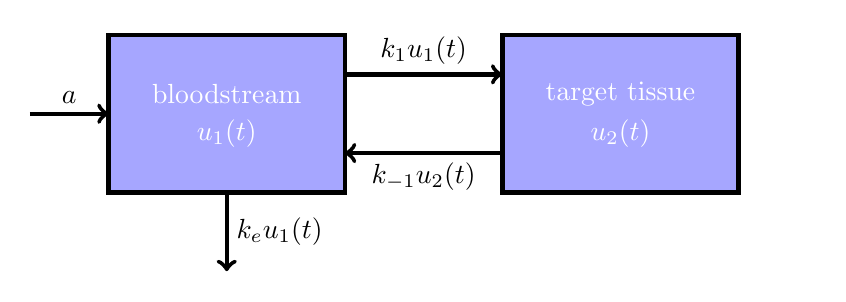
\begin{tikzpicture}
    \filldraw[blue!35] (0,0)--(3,0)--(3,2)--(0,2)--cycle;
    \filldraw[blue!35] (5,0)--(8,0)--(8,2)--(5,2)--cycle;
    \draw[ultra thick] (0,0)--(3,0)--(3,2)--(0,2)--cycle;
    \draw[ultra thick] (5,0)--(8,0)--(8,2)--(5,2)--cycle;
    \draw[->, ultra thick] (-1,1) -- (0,1);
    \node[above] at (-0.5,1) {\(a\)};
    \draw[white] (8.1,1)--(9,1);
    \draw[->, ultra thick] (3,1.5)--(5,1.5);
    \node[above] at (4,1.5) {\(k_1 u_1(t)\)};
    \draw[->, ultra thick] (5,0.5)--(3,0.5);
    \node[below] at (4,0.5) {\(k_{-1} u_2(t)\)};
    \draw[->, ultra thick] (1.5,0) -- (1.5,-1);
    \node[right] at (1.5,-0.5) {\(k_e  u_1(t)\)};
    \node[white] at (1.5, 1.25) {bloodstream};
    \node[white] at (1.5, 0.75) {\(u_1(t)\)};
    \node[white] at (6.5, 1.25) {target tissue};
    \node[white] at (6.5, 0.75) {\(u_2(t)\)};
  \end{tikzpicture}
\end{center} 

From the picture \(u_1(t)\) and \(u_2(t)\) satisfy
\begin{equation}\label{eq:sys-45}
\begin{array}{lcrcc}
  u_1'(t) &=& - 0.009  u_1(t) + 0.003 u_2(t) &+& 0.6\\
  u_2'(t) &=& 0.007  u_1(t) - 0.003 u_2(t) 
\end{array}
\end{equation}
We identify an equilibrium by first setting \(u_1'(t) = u_2'(t) = 0\), \(u_1(t) = u_1^*\), and \(u_2(t) =u_2^*\) to obtain
\begin{equation}\label{eq:sys-46}
\begin{array}{lcrcc}
  0 &=& - 0.009  u_1^* + 0.003 u_2^* &+& 0.6\\
  0 &=& 0.007  u_1^* - 0.003 u_2^* 
\end{array}
\end{equation}
Solving the system we find the equilibrium to be \(\vec{u}^{ *} = \begin{bmatrix} 300 \\ 700 \end{bmatrix}\).

We now define \(\vec{x}(t)\) as \(\begin{bmatrix} u_1(t) \\ u_2(t) \end{bmatrix} -\begin{bmatrix} 300 \\ 700 \end{bmatrix}\). Then we look to solve
\begin{equation}\label{eq:sys-47}
\vec{x}'(t) =
\begin{bmatrix}
  -0.009 & 0.003 \\
  0.007 & -0.003
\end{bmatrix}
\vec{x}(t)
\quad
\text{with}
\quad
\vec{x}(0) =
\begin{bmatrix}
  -300 \\ -700
\end{bmatrix}.
\end{equation}
The matrix in the preceding homogeneous equation has two distinct real eigenvalues. In fact, the eigenvalue-eigenvector pairs are
\begin{equation}\label{eq:sys-48}
\lambda_1 =
\frac{-6 + \sqrt{30}}{1000}, \quad \vec{v}_1 = \begin{bmatrix} 3 \\ 3 +\sqrt{30} \end{bmatrix}
\end{equation}
and
\begin{equation}\label{eq:sys-49}
\lambda_2 =
\frac{-6 - \sqrt{30}}{1000}, \quad \vec{v}_2 = \begin{bmatrix} 3 \\ 3 -\sqrt{30} \end{bmatrix}
\end{equation}
Using the initial condition we find that
\begin{equation}\label{eq:sys-50}
\vec{x}(t)
=
-\left(\frac{20\sqrt{30}}{3} + 50\right)  e^{\lambda_1 t} \begin{bmatrix} 3 \\ 3 +\sqrt{30} \end{bmatrix}
+
\left(\frac{20\sqrt{30}}{3} - 50\right) e^{\lambda_2 t} \begin{bmatrix} 3 \\ 3 -\sqrt{30} \end{bmatrix}
\end{equation}
and so
\begin{multline}\label{eq:sys-51}
  \begin{bmatrix} u_1(t) \\ u_2(t) \end{bmatrix} = 
  \begin{bmatrix} 300 \\ 700 \end{bmatrix} 
  -\left(\frac{20\sqrt{30}}{3} + 50\right)  e^{\lambda_1 t} \begin{bmatrix} 3 \\ 3 +\sqrt{30} \end{bmatrix}
  \\[1ex]+
  \left(\frac{20\sqrt{30}}{3} - 50\right) e^{\lambda_2 t} \begin{bmatrix} 3 \\ 3 -\sqrt{30} \end{bmatrix}.
\end{multline}
Because \(\lambda_1, \lambda_2 < 0\) we can also see that the equilibrium solution we identified is asymptotically stable.
\end{solution}

As we said, the strategy for solving \eqref{eq:inhomog} by re-defining variables relative to an equilibrium is quite straightforward. However, we can only be sure that an equilbrium \(\vec{u}^{ *}\) exists when zero is \emph{not} an eigenvalue of \(A\).

When zero is an eigenvalue of \(A\), an equilibrium will only exist when \(\vec{b}\) is an eigenvector associated with the other (non-zero) eigenvalue \(\lambda\). In this case, \(\vec{u}^{ *} = -\vec{b}/\lambda\) would be the equilibrium and we can use the strategy for finding a solution outlined above.

When zero is an eigenvalue of \(A\) and \(\vec{b}\) is not an eigenvector associated with the other eigenvalue, then a different strategy for finding a solution is required because no equilibrium exists. The path forward in this case is a bit complicated, but is not beyond our grasp. To understand the procedure, we first define the \emph{transpose of \(A\)}, denoted \(A^T\), as the matrix whose \(i\)th row is the \(i\)th column of \(A\). As an example, if \(A = \begin{bmatrix} a & b \\ c & d\end{bmatrix}\) then \(A^T = \begin{bmatrix}a & c \\ b & d \end{bmatrix}\).

It can be shown that \(A\) and \(A^T\) have the same eigenvalues,\footnote{One can easily verify this directly for the case in which \(A\) is \(2\times 2\) matrix.} though their eigenvectors may differ. That said, we approach the next step in the process by focusing on an eigenvector of \(A^T\) that is associated with the zero eigenvalue of the matrix. Let \(\vec{v}\) denote this eigenvector, and define a new variable \(y(t) = \vec{v}\bullet \vec{u}(t)\) where \(\vec{u}(t)\) is the solution to the given inhomogeneous differential equation. It follows that
\begin{equation}\label{eq:sys-52}
y'(t) = \vec{v} \bullet \vec{u}^{ \prime}(t) 
= \vec{v} \bullet ( A \vec{u}(t) + \vec{b} )
= \vec{v} \bullet A \vec{u}(t) + \vec{v} \bullet \vec{b}
= \vec{u}(t) \bullet A^T \vec{v} + \vec{v} \bullet \vec{b}
= \vec{v} \bullet \vec{b}
\end{equation}
where we have applied a well-known identity to convert \(\vec{v} \bullet A \vec{u}(t)\) to \(\vec{u}(t) \bullet A^T \vec{v} = 0\). Solving the equation we arrive at
\begin{equation}\label{eq:sys-53}
y(t) = \vec{v}\bullet\vec{b} t + \vec{v}\bullet\vec{u}(0)
\quad\leftrightarrow\quad
v_2 u_2(t) + v_1  u_1(t) =
\vec{v}\bullet\vec{b} t + \vec{v}\bullet\vec{u}(0)
\end{equation}
which can be used to turn the given system of equations into a single linear equation that we can solve using the approaches set out in Chapter 2. The next example shows how our alternative strategy works, in practice.

\begin{example} \label{eg:ivp1}
Solve the initial-value problem
\begin{equation}\label{eq:sys-54}
\frac{d}{dt} \vec{u}(t)
=
\begin{bmatrix} 2 & 1 \\ 4 & 2 \end{bmatrix} \vec{u}(t) + \begin{bmatrix} 3 & 1 \end{bmatrix}
\quad
\text{with}
\quad
\vec{u}(0) = \begin{bmatrix} 1 & 1 \end{bmatrix}
\end{equation}
\end{example}

% solution to eg:ivp1
\begin{solution}
The matrix featured in the differential equation has a zero eigenvalue, associated with an eigenvector \(\begin{bmatrix} 1 \\ -2 \end{bmatrix}\). Since \(\begin{bmatrix} 3 \\ 1 \end{bmatrix}\) is not a multiple of this eigenvalue, we cannot find an equilibrium solution to the differential equation. We therefore try our alternate approach.

The transpose of the matrix from the differential equation is \(\begin{bmatrix} 2 & 4 \\ 1 & 2 \end{bmatrix}\). It also has a zero eigenvalue, but this eigenvalue is associated with an eigenvector \(\vec{v} = \begin{bmatrix} -2 \\ 1 \end{bmatrix}\).

Define \(y(t) = \vec{v} \bullet \vec{u}(t)\) and observe that
\begin{equation}\label{eq:sys-55}
\begin{aligned}
  y'(t) 
  &= -2  u_1'(t) + u_2'(t) \\
  &= -2(2 u_1(t) + u_2(t) +3) +(4u_1(t) + 2 u_2(t) + 1) \\
  &= - 5 .
\end{aligned}
\end{equation}
Using the fact that \(y(0) = \vec{v} \bullet\vec{u}(0) = -1\) we get
\begin{equation}\label{eq:sys-56}
y(t) = - 5 t - 1
\quad\longrightarrow\quad
u_2(t) = 2 u_1(t) - 5 t - 1.
\end{equation}
Substituting the previous expression into the differential equation we have been given for \(u_1(t)\) we obtain
\begin{equation}\label{eq:sys-57}
u_1'(t) = 2 u_1(t) + (2 u_1(t) - 5 t - 1) + 3
\quad\longleftrightarrow\quad
u_1'(t) - 4 u_1(t) = 2 - 5 t
\end{equation}
with \(u_1(0)=1\). We find
\begin{equation}\label{eq:sys-58}
u_1(t) = e^{4 t} + e^{4 t}  \int_{0}^{t} e^{-4 s} (2-5 s) ds
\end{equation}
and so
\begin{equation}\label{eq:sys-59}
u_2(t) = 2 e^{4 t} + 2 e^{4 t} \int_0^t e^{-4 s} (2-5 s) ds 5t -1.
\end{equation}
\end{solution}

There is so much more to say about systems of differential equations. In fact, most universities offer several courses on differential equations at the undergraduate level alone. Later courses outline the various ways in which models can simultaneously incorporate changes that occur over both time and space. More advanced treatments provide modellers with strategies for coping with the non-linear feedbacks we saw in the predator-prey model we tackled at the outset of this chapter.  Some courses focus on computational strategies while others emphasize analytic ``pencil and paper'' methods. Though these topics are beyond the scope of this text, they are surely not beyond the scope of its readers' ability.

\end{document}
